\begin{table*}[h]\centering
\begin{tabular}{|l|c|c|c|c|c|}
\hline
                            & PQL2 & PQL3 & PQL+ & WQSP & CWQ \\
\hline
KV-MemNN \cite{DBLP:conf/emnlp/MillerFDKBW16}    & 72.2 & 67.4 & -    & 46.7 / - & 21.1\footnote{The original paper only reports scores on development set.} / -      \\
IRN \cite{DBLP:conf/coling/ZhouHZ18}                         & 72.5 & 71.0   & 52.9 & -    & -         \\
HR-BiLSTM \cite{DBLP:conf/acl/YuYHSXZ17}                  & 97.5 & 87.9 & 92.9 & 62.9 / 62.3 & 33.3 / 31.2         \\
ABWIM \cite{DBLP:journals/corr/abs-1801-09893}                      & 94.3 & 89.3 & 92.6 & -    & -         \\
UHop\footnote{We use the best reported setup from the original paper, aka. ABWIM with UHop.} \cite{DBLP:conf/naacl/ChenCCNK19}                       & 97.5 & 89.3 & 92.3 & -    & -         \\
GRAFT-Net \cite{DBLP:conf/emnlp/SunDZMSC18}                  & -    & -    & -    & 67.8 / 62.5 & 30.1 / 26.0      \\
KBQA with Topic Units \cite{DBLP:conf/ijcai/LanW019}                  & -    & -    & -    & 68.2 / 67.9 & 39.3 / 36.5      \\
\hline
Our Method-obj1             & 98.3 & 97.1 & 97.5 &    62.8 / 62.3  &           \\
Our Method-obj2             &   -   &   -   &   -   &  65.4 / 65.1     &           \\
Our Method-obj3             &     - &  -    &   -   &   67.9 / 67.0    &           \\
Our Method-obj3+new\_decode & -     &   -   &    -   &     &          \\
\hline
\end{tabular}
\caption{\fontsize{10}{12}\selectfont We report Accuracy on PQL and hits@1 and F1 on WQSP and CWQ. All scores except our method are copied from the previous published papers. obj1/2: $P(ans, path|x)= P(ans|path,x)*P(path|x)$ with single/multiple reasoning paths for one sample. obj3: $P(ans) = sum_path(P(ans|path,x)*P(path|x))$, new\_decode: use beam search and multi paths in decoding.}\label{tab:main}
\end{table*}


\begin{figure}[h]
\centering
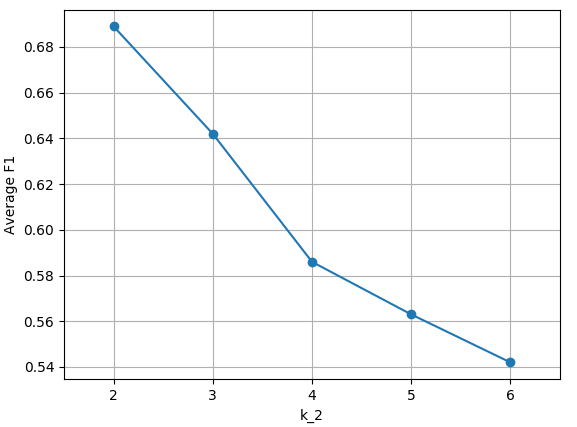
\includegraphics[width=0.85\columnwidth]{figs/fig2.png}
\vspace{-2ex}
\caption{\fontsize{10}{12}\selectfont Average F1 over different thresholds on \textsc{WebQuestionSp} dataset.}
\label{fig:k2}
\end{figure}


\begin{table}[h]\centering
\resizebox{1.01\columnwidth}{!}{
\begin{tabular}{|l|c|c|}
\hline
                           & WQSP & CWQ \\
\hline
%KV-MemNN \cite{DBLP:conf/emnlp/MillerFDKBW16}    & 46.7 / - & 21.1\tablefootnote{The original paper only reports scores on development set.} / -      \\
HR-BiLSTM \cite{DBLP:conf/acl/YuYHSXZ17}                  & 62.9 / 62.3 & 33.3 / 31.2         \\
GRAFT-Net \cite{DBLP:conf/emnlp/SunDZMSC18}                & 67.8 / 62.5 & 30.1 / 26.0      \\
KBQA-GST \cite{DBLP:conf/ijcai/LanW019}          & 68.2 / 67.9 & 39.3 / \textbf{36.5}      \\
\hline
Our Method-joint\_prob             &    62.8 / 62.3  &   36.7 / 31.4        \\
Our Method-joint\_prob\_multiple\_paths             &  65.4 / 65.1     &    - / -       \\
Our Method-marginal\_prob\_with\_true\_label             &   \textbf{68.9} / \textbf{68.5}    &      \textbf{39.4} / 34.8     \\
Our Method-marginal\_prob\_without\_true\_label             &   68.8 / 68.3    &       33.0 / 27.6    \\
%Our Method-obj3+new\_decode  &     &          \\
\hline
\end{tabular}
}
\caption{\fontsize{10}{12}\selectfont We report hits@1 / F1 on WQSP and CWQ.}\label{tab:wqsp_cwq}
\end{table}


A general neural network solution to KBQA is to encode the candidates of relation path or answer into embeddings, and choose or rank these embeddings based on different ranking functions. Existing approaches can be categorized into three types. One is to match the question to a candidate directly via calculating the similarity between them \cite{DBLP:journals/corr/abs-1801-09893,DBLP:conf/adbis/YuHYZW18}. This method is not very suitable for multi-hop questions with long paths, because the number of candidate entity-relation combinations grows exponentially as the number of hops increases. The second type of algorithms is to encode the reasoning information hop by hop, and predict the final answer at the last hop \cite{DBLP:conf/emnlp/MillerFDKBW16,DBLP:conf/coling/ZhouHZ18}, which is a group of methods that are more capable of handling multi-hop questions. Most of these algorithms, however, are restricted to a fixed maximum number of hops, and this number is normally chosen as a relative small number. Recently, a new unrestricted-hop framework is proposed to dynamically choose the number of hops to be executed, by introducing a ``stop'' action to decide when is the last hop \cite{DBLP:conf/naacl/ChenCCNK19}. The third type is specifically designed for multi-hop KBQA, which decompose the input question into several single-hop question, and use the exiting method to solve each simple question. The decomposition methods are based on semantic parsing \cite{DBLP:conf/www/AbujabalYRW17,DBLP:conf/emnlp/LuoLLZ18}, pointer network \cite{DBLP:conf/acl/MinZZH19}, or predefined templates \cite{DBLP:journals/pvldb/ZhengYZC18,DBLP:journals/corr/abs-1807-09623}.  %This number is normally chosen as a relative small number like 1 (single hop), 2 or 3. One main reason is because that, despite theoretically it is possible to search all the possible relations greedily and find the paths starting from the focus entity in the question to the answer entity, the number of all possible entity-relation combinations grows exponentially. It is unrealistic to store or even enlist all these paths when the number of hops is too large. Moreover, it is also unlikely for the system to know the number of hops in advance in real applications. 
 To further improve a multi-hop KBQA system's performance, some recent work also replaces the standard entity linking module by leveraging an augmented topic entity candidate pool \cite{DBLP:conf/ijcai/LanW019}, such that it can cover more entity possibilities. This work is similar to our idea that making use of multiple input information to train the model, but their focus is on entities while ours is on relation paths.
%\kechen{add relation prediction references and multiple relation path, recent ijcai paper?}



\kechen{should we move this to RW? Most of the existing multi-hop KBQA systems \cite{DBLP:conf/acl/YuYHSXZ17,DBLP:journals/corr/abs-1801-09893,DBLP:conf/coling/ZhouHZ18,DBLP:conf/naacl/ChenCCNK19} approach this task by decomposing it into two sub-tasks:
%Currently, there are mainly two main categories of methods to tackle the complex KBQA problems, the first category is based on semantic parsing, and the other category mainly relies on the embeddings (XXX) for information retrieval (IR). %Their differences will be discussed further in the relation work section, and i
%In this paper, we focus on the second category, \emph{i.e.} the embedding based approach, which can either predict the answer directly (XXX) or search (a) relation path(s) leading to the final answer entity (XXX). Conventionally, the relation path searching algorithm consists two main subtasks
topic/focus--entity linking and relation extraction. The topic--entity linking gives the system an entry point to start searching, and the relation extraction is used to search relation paths leading to the final answer. %Unlike the simple single relation questions, for complex questions, the path to the final answer may contains multiple hops, where one hop is defined as a searching step between one entity to another via a single relation. 
For entity linking, there exists many off-the-shell tools  \cite{DBLP:journals/corr/YangC16a} that can give decent performance, and most of the current KBQA models rely on them. For relation extraction, traditional approaches consider all the paths as candidates and search for the best one among them using ranking algorithms.}